\section{Strumentazione}
	In questa esperienza si sono impiegati :	
	\begin{list}{$\cdot$}
	\item un tetrodo a gas neon ELWE U84822330
	\item un sistema di alimentazione e 
		lettura di corrente ELWE
	\item un oscilloscopio
	\end{list}
\subsection{Descrizione dell'apparato sperimentale}
	Il tetrodo a gas si costituisce 
	di un tubo elettronico nel quale �
	presente un gas rarefatto in cui sono disposti 4 elettrodi.
	Per il tetrodo in utilizzo il 
	gas impiegato � il neon, ad 
	una pressione di $\sim$\SI{10}{e{-3} \bar}.
	I quattro elettrodi sono chiamati catodo,griglia di 
	controllo
	griglia d'anodo e collettore.
	
	Il catodo costituisce la sorgente di elettroni,infatti il 
	catodo riscaldandosi sino al calore rosso per effetto 
	termoionico 
	emette elettroni, di energia trascurabile rispetto a quelle
	impiegate in questa esperienza(per il calor rosso 
	$\sim$ \SI{1000}{\kelvin} si ottiene
	$KT \sim$ \SI{0.1}{\electronvolt}).
	Le griglie sono costituite da due conduttori fatti in 
	una rete
	di fili sottili.
	Tale geometria � tale da permettere il passaggio 
	degli elettroni attraverso la griglia
	e da costituire per le approssimazioni impiegate un piano equipotenziale.
	
	Il tetrodo � collegato al dispositivo di alimentazione;
	tale dispositivo permette di regolare la tensione
	\begin{itemize}
		\item $U_F$ tensione impiegata per riscaldare il catodo 
			e regolare il rate di emissione degli $e^{-}$
		\item $U_G$ differenza di potenziale fra la griglia di 
			controllo
			e la griglia catodo in modo da aumentare l'emissivit�
		\item $U_A$ costituisce il campo 
			accelerante per gli $e^{-}$
			fuoriusciti dalla griglia di controllo
		\item $U_E$ le la differenza di potenziale applicata 
			fra griglia anodica e collettore.Costituisce il campo frenante
			per gli elettroni che fuoriescono dal collettore.
	\end{itemize}
	Essendo che le misure effettuate attraverso 
	l'oscilloscopio sono misure di tensione 
	per convertire la corrente $I_C$ nel 
	collettore
	� stato collegato a un amplificatore a 
	transimpedenza.
	DA CONTROLLARE SE VERO -NON ERA IL CIRCITO STAMPATO IN FIGRA S L'ACCROCCHIO CON LE MANOPOLE?-
	
	
	\bigskip
	\begin{figure} [!h]
		\centering
		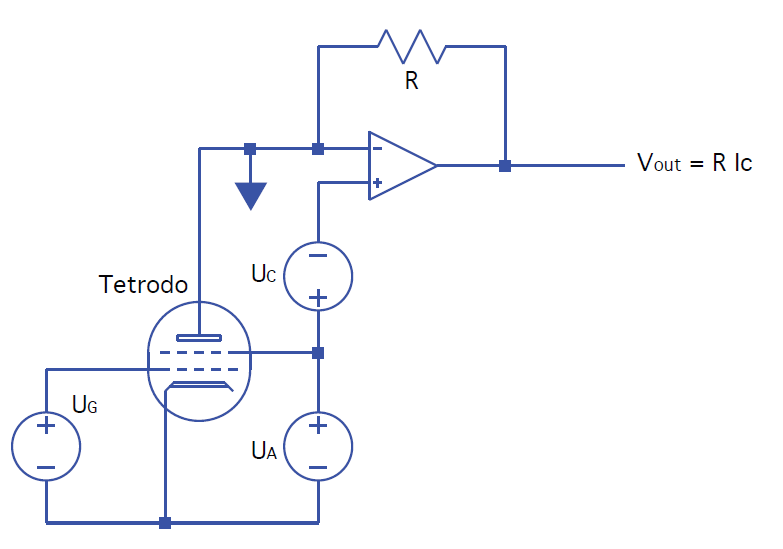
\includegraphics[width=0.9\textwidth]{./fig/apparato.png}
		\caption{Schema dell'apparato impiegato.}
		\label{fig:apparato}
	\end{figure}
	
	Si riporta in \fig{fig:apparato} uno schema 
	dell'apparato sperimentale impiegato. 
	